\section*{Analyse}
\label{Analyse}
%
Før analysen udføres, opstilles et boksplot for hver af de fire hovedpositioner, jævnfør \autoref{fig:boksplot}. Baseret på \autoref{fig:boksplot} tyder det på, at position 2 og position 3 begge perciperes som værende mere indbydende sammenlignet med position 1 og position 4.   
%
\begin{figure}[H]
\centering
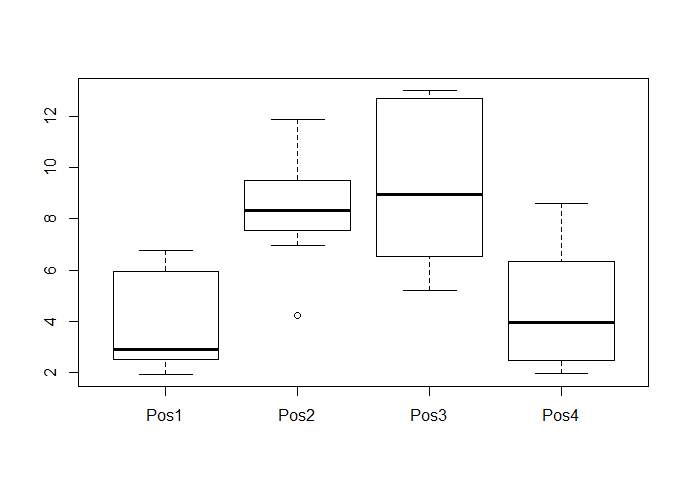
\includegraphics[width = 0.7\textwidth]{Figure/Rplot.png} 
\caption{Boksplot over hvor indbydende hver af de fire hovedpositioner perciperes.}
\label{fig:boksplot}
\end{figure}
\noindent
%
Data analyseres med en \textit{one-way repeated measures ANOVA}, \parencite[s. 554]{DiscoveringStatisticsUsingR}. Hvor \textit{one-way} refererer til antallet af uafhængige variable, som i dette tilfælde er én; robottens hovedposition. \textit{Repeated measures} refererer til, at samtlige testpersoner præsenteres for samtlige stimuli. Da formålet med denne test er at undersøge hvor indbydende en robot perciperes afhængigt af dens hovedposition, er den afhængige variabel testpersonernes individuelle respons angivet på skalaen. Den indsamlede data er af typen interval data, hvilket skyldes at VAS er en kontinuerlig skala. 

Ydermere dækker den uafhængige variabel over fire kategorier; de fire forskellige hovedpositioner, er det ligeledes oplagt at anvende en ANOVA, da det ønskes at sammenligne mere end to kategorier.\blankline
%
Følgende antagelser skal overholdes for at udføre en \textit{one-way repeated measures ANOVA}: \blankline  
%
\begin{itemize}
	\item \textbf{Den afhængige variabel skal som minimum være målt på interval skala.}\\
	Vurderingen givet på skalaen er målt på en interval skala og opfylder dermed denne antagelse.
	\item \textbf{Der skal være homogen varians. }\\
	For at teste om der er homogen varians udføres \textit{Levene's test}. Testresultatet er $F(3.28)=1.09, p=0.37$, hvorfor der ikke er signifikant forskel og dermed er antagelsen om homogen varians opfyldt. 
	\item \textbf{Data skal være normalfordelt.}\\
	For teste om der er normalfordeling udføres en \textit{Shapiro-Wilk test}. Testresultatet er $W=0.94, p=0.09$, hvorfor der ikke er signifikant forskel og dermed er antagelsen om normalfordeling er opfyldt.\blankline
\end{itemize}
\noindent
%
Da alle antagelser for at udføre en \textit{one-way repeated measures ANOVA} er opfyldt, udføres denne i \textit{rStudio}. Testresultatet er $F(3.21)=13,7, p=4.4*e^{-4}$, hvilket indikerer at der er signifikant effekt af robottens hovedposition på hvor indbydende robotten perciperes.
%HER TIL!!% 

Analysen viser at der er en forskel, men ikke mellem hvilke positioner forskellen er. For at undersøge hvor forskellen er, udføres der post hoc test, mere specifikt den type der hedder \textit{pairwise comparisons using t-tests}. Resultatet af denne test kan ses i \autoref{fig:sammenligning}.
\begin{figure}[H]
\centering
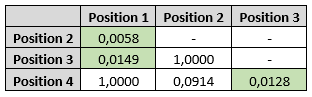
\includegraphics[width = 0.5\textwidth]{Figure/PostHocExcel.PNG} 
\caption{Sammenligning mellem vurderingerne afgivet til hver position. Grøn markering angiver at der er signifikant forskel.}
\label{fig:sammenligning}
\end{figure}

\noindent Resultatet viser at både position 2 og 3 er signifikant forskellige fra position 1. Ud fra boksplottene på \autoref{fig:boksplot} konkluderes det at position 2 og 3 må være vurderet signifikant højere end position 1, og derved blevet opfattet som mere indbydende. 
\\\\
Der er ligeledes signifikant forskel mellem position 3 og 4. Det er værd at bemærke at der ikke er signifikant forskel mellem vurderingen af position 2 og 4. 